\problemname{Fixing Fractions}

\illustration{0.3}{meme.png}{Source: The Internet\texttrademark.\vspace{-6em}}%
Maths is hard.\textsuperscript{[citation needed]}
But it could be easier!
And the internet\texttrademark{} has found some excellent ways to make it easier.
Take a look at the following true equations:
\begin{center}
    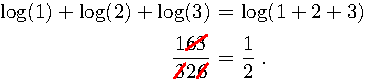
\includegraphics{fraction1.pdf}
\end{center}\vspace{-0.5\baselineskip}
Following the patterns, we come to the conclusion that the following equation should also be true:\vspace{-0.75\baselineskip}
\begin{center}
    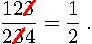
\includegraphics{fraction2.pdf}
\end{center}\vspace{-0.5\baselineskip}
However, this is actually wrong in boring old standard maths.
Therefore, we define a new kind of funky maths where it is allowed to cancel out digits on the left side of the equality sign.
This surely will make everyone's life easier.
Except yours, since you have to evaluate if two given fractions are equal in our new funky maths.

%		Note that the following equation is still wrong in our new maths:
%		\begin{align*}
%			\frac{1}{2}&\neq\frac{123}{234}~.
%		\end{align*}
\begin{Input}
The input consists of:
\begin{itemize}
\item One line with four integers $a$, $b$, $c$, and $d$ ($1\leq a,b,c,d<10^{18}$), describing the two fractions $\frac{a}{b}$ and $\frac{c}{d}$.
\end{itemize}
\end{Input}

\begin{Output}
If there exist integers $a'$ and $b'$ obtained from $a$ and $b$ by cancelling
out the same digits and with $\frac{a'}{b'} = \frac{c}{d}$ in standard mathematics, output
``\texttt{possible}'', followed by $a'$ and $b'$.
Otherwise, output ``\texttt{impossible}''.

If there are multiple valid solutions, you may output any one of them.

Note that neither $a'$ nor $b'$ is allowed to contain leading zeroes after
cancelling digits.
\end{Output}
